\documentclass[class=minimal,border=0pt]{standalone}
\usepackage{hyperref}
\hypersetup{
colorlinks=true,
urlcolor=cyan}
\usepackage{tikz}
\begin{document}
%\documentclass{standalone}
%\usepackage{tikz}
%\usetikzlibrary{patterns,plotmarks}
%\begin{document}
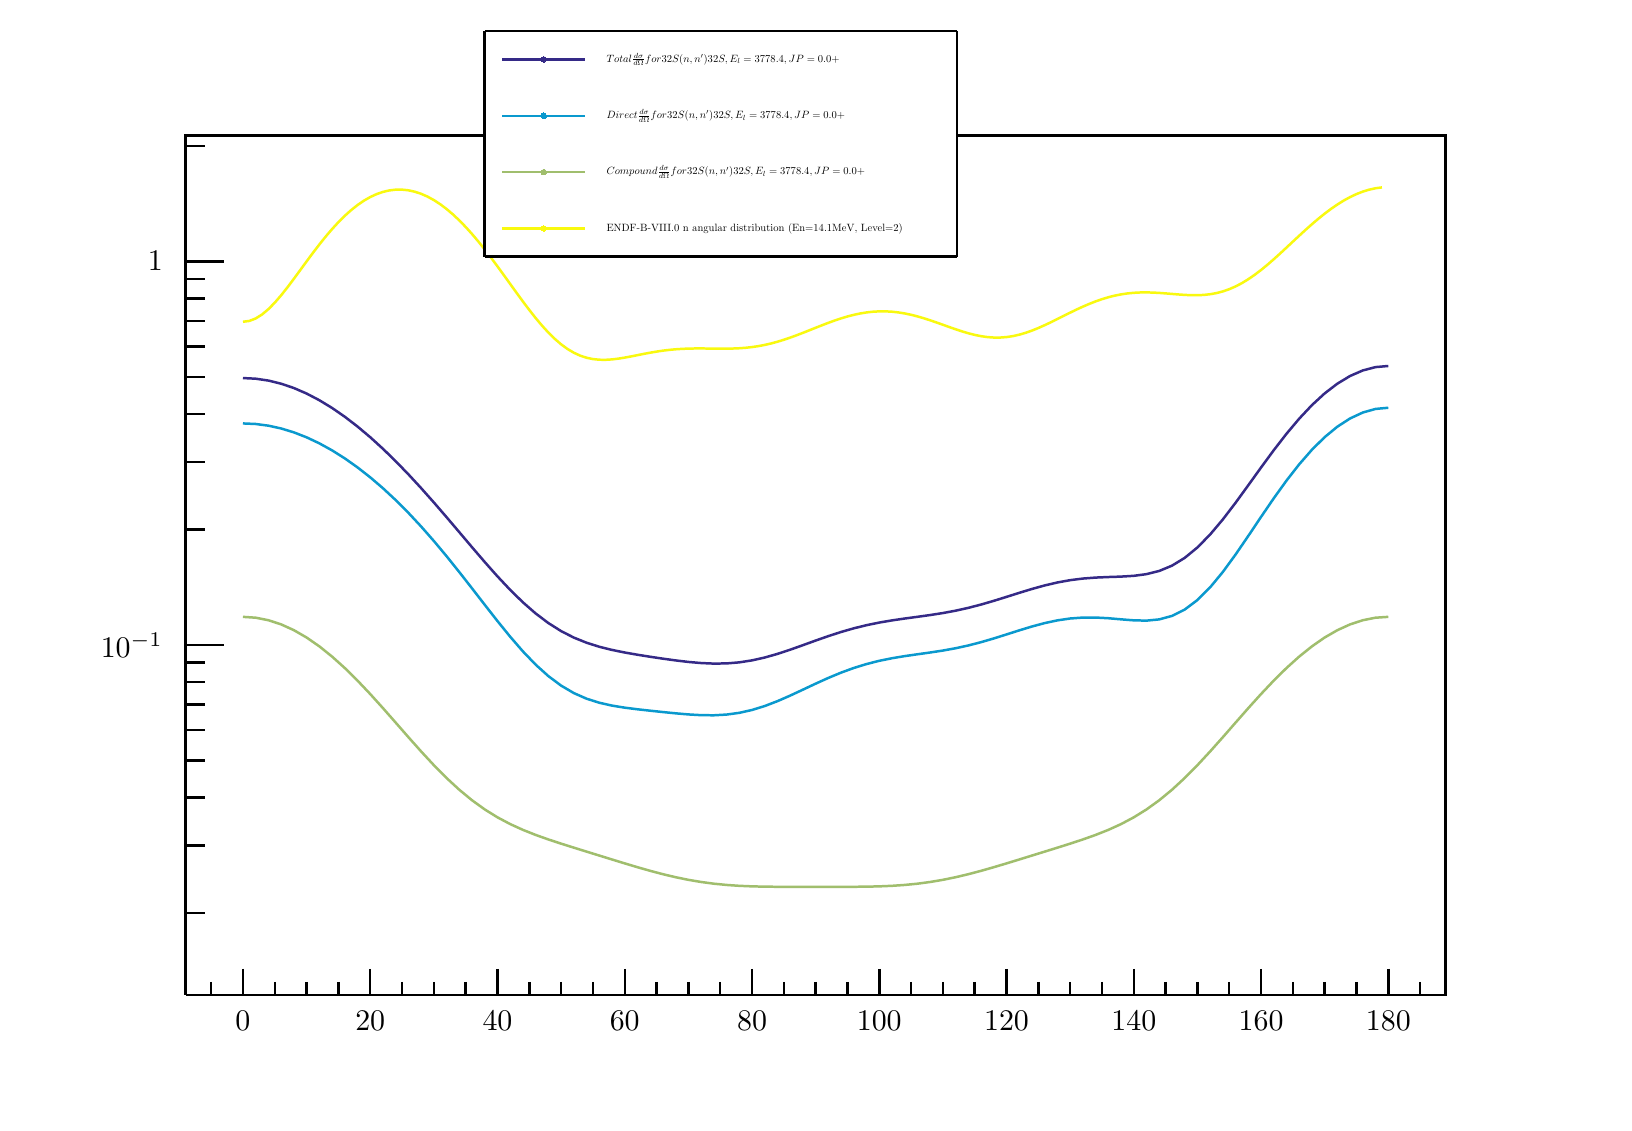
\begin{tikzpicture}
\def\CheckTikzLibraryLoaded#1{ \ifcsname tikz@library@#1@loaded\endcsname \else \PackageWarning{tikz}{usetikzlibrary{#1} is missing in the preamble.} \fi }
\CheckTikzLibraryLoaded{patterns}
\CheckTikzLibraryLoaded{plotmarks}
\pgfdeclareplotmark{cross} {
\pgfpathmoveto{\pgfpoint{-0.3\pgfplotmarksize}{\pgfplotmarksize}}
\pgfpathlineto{\pgfpoint{+0.3\pgfplotmarksize}{\pgfplotmarksize}}
\pgfpathlineto{\pgfpoint{+0.3\pgfplotmarksize}{0.3\pgfplotmarksize}}
\pgfpathlineto{\pgfpoint{+1\pgfplotmarksize}{0.3\pgfplotmarksize}}
\pgfpathlineto{\pgfpoint{+1\pgfplotmarksize}{-0.3\pgfplotmarksize}}
\pgfpathlineto{\pgfpoint{+0.3\pgfplotmarksize}{-0.3\pgfplotmarksize}}
\pgfpathlineto{\pgfpoint{+0.3\pgfplotmarksize}{-1.\pgfplotmarksize}}
\pgfpathlineto{\pgfpoint{-0.3\pgfplotmarksize}{-1.\pgfplotmarksize}}
\pgfpathlineto{\pgfpoint{-0.3\pgfplotmarksize}{-0.3\pgfplotmarksize}}
\pgfpathlineto{\pgfpoint{-1.\pgfplotmarksize}{-0.3\pgfplotmarksize}}
\pgfpathlineto{\pgfpoint{-1.\pgfplotmarksize}{0.3\pgfplotmarksize}}
\pgfpathlineto{\pgfpoint{-0.3\pgfplotmarksize}{0.3\pgfplotmarksize}}
\pgfpathclose
\pgfusepathqstroke
}
\pgfdeclareplotmark{cross*} {
\pgfpathmoveto{\pgfpoint{-0.3\pgfplotmarksize}{\pgfplotmarksize}}
\pgfpathlineto{\pgfpoint{+0.3\pgfplotmarksize}{\pgfplotmarksize}}
\pgfpathlineto{\pgfpoint{+0.3\pgfplotmarksize}{0.3\pgfplotmarksize}}
\pgfpathlineto{\pgfpoint{+1\pgfplotmarksize}{0.3\pgfplotmarksize}}
\pgfpathlineto{\pgfpoint{+1\pgfplotmarksize}{-0.3\pgfplotmarksize}}
\pgfpathlineto{\pgfpoint{+0.3\pgfplotmarksize}{-0.3\pgfplotmarksize}}
\pgfpathlineto{\pgfpoint{+0.3\pgfplotmarksize}{-1.\pgfplotmarksize}}
\pgfpathlineto{\pgfpoint{-0.3\pgfplotmarksize}{-1.\pgfplotmarksize}}
\pgfpathlineto{\pgfpoint{-0.3\pgfplotmarksize}{-0.3\pgfplotmarksize}}
\pgfpathlineto{\pgfpoint{-1.\pgfplotmarksize}{-0.3\pgfplotmarksize}}
\pgfpathlineto{\pgfpoint{-1.\pgfplotmarksize}{0.3\pgfplotmarksize}}
\pgfpathlineto{\pgfpoint{-0.3\pgfplotmarksize}{0.3\pgfplotmarksize}}
\pgfpathclose
\pgfusepathqfillstroke
}
\pgfdeclareplotmark{newstar} {
\pgfpathmoveto{\pgfqpoint{0pt}{\pgfplotmarksize}}
\pgfpathlineto{\pgfqpointpolar{44}{0.5\pgfplotmarksize}}
\pgfpathlineto{\pgfqpointpolar{18}{\pgfplotmarksize}}
\pgfpathlineto{\pgfqpointpolar{-20}{0.5\pgfplotmarksize}}
\pgfpathlineto{\pgfqpointpolar{-54}{\pgfplotmarksize}}
\pgfpathlineto{\pgfqpointpolar{-90}{0.5\pgfplotmarksize}}
\pgfpathlineto{\pgfqpointpolar{234}{\pgfplotmarksize}}
\pgfpathlineto{\pgfqpointpolar{198}{0.5\pgfplotmarksize}}
\pgfpathlineto{\pgfqpointpolar{162}{\pgfplotmarksize}}
\pgfpathlineto{\pgfqpointpolar{134}{0.5\pgfplotmarksize}}
\pgfpathclose
\pgfusepathqstroke
}
\pgfdeclareplotmark{newstar*} {
\pgfpathmoveto{\pgfqpoint{0pt}{\pgfplotmarksize}}
\pgfpathlineto{\pgfqpointpolar{44}{0.5\pgfplotmarksize}}
\pgfpathlineto{\pgfqpointpolar{18}{\pgfplotmarksize}}
\pgfpathlineto{\pgfqpointpolar{-20}{0.5\pgfplotmarksize}}
\pgfpathlineto{\pgfqpointpolar{-54}{\pgfplotmarksize}}
\pgfpathlineto{\pgfqpointpolar{-90}{0.5\pgfplotmarksize}}
\pgfpathlineto{\pgfqpointpolar{234}{\pgfplotmarksize}}
\pgfpathlineto{\pgfqpointpolar{198}{0.5\pgfplotmarksize}}
\pgfpathlineto{\pgfqpointpolar{162}{\pgfplotmarksize}}
\pgfpathlineto{\pgfqpointpolar{134}{0.5\pgfplotmarksize}}
\pgfpathclose
\pgfusepathqfillstroke
}
\definecolor{c}{rgb}{1,1,1};
\draw [color=c, fill=c] (0,0) rectangle (20,13.639);
\draw [color=c, fill=c] (2,1.3639) rectangle (18,12.2751);
\definecolor{c}{rgb}{0,0,0};
\draw [c,line width=0.9] (2,1.3639) -- (2,12.2751) -- (18,12.2751) -- (18,1.3639) -- (2,1.3639);
\draw [c,line width=0.9] (2,1.3639) -- (18,1.3639);
\draw [c,line width=0.9] (2.72727,1.69123) -- (2.72727,1.3639);
\draw [c,line width=0.9] (3.13131,1.52756) -- (3.13131,1.3639);
\draw [c,line width=0.9] (3.53535,1.52756) -- (3.53535,1.3639);
\draw [c,line width=0.9] (3.93939,1.52756) -- (3.93939,1.3639);
\draw [c,line width=0.9] (4.34343,1.69123) -- (4.34343,1.3639);
\draw [c,line width=0.9] (4.74747,1.52756) -- (4.74747,1.3639);
\draw [c,line width=0.9] (5.15152,1.52756) -- (5.15152,1.3639);
\draw [c,line width=0.9] (5.55556,1.52756) -- (5.55556,1.3639);
\draw [c,line width=0.9] (5.9596,1.69123) -- (5.9596,1.3639);
\draw [c,line width=0.9] (6.36364,1.52756) -- (6.36364,1.3639);
\draw [c,line width=0.9] (6.76768,1.52756) -- (6.76768,1.3639);
\draw [c,line width=0.9] (7.17172,1.52756) -- (7.17172,1.3639);
\draw [c,line width=0.9] (7.57576,1.69123) -- (7.57576,1.3639);
\draw [c,line width=0.9] (7.9798,1.52756) -- (7.9798,1.3639);
\draw [c,line width=0.9] (8.38384,1.52756) -- (8.38384,1.3639);
\draw [c,line width=0.9] (8.78788,1.52756) -- (8.78788,1.3639);
\draw [c,line width=0.9] (9.19192,1.69123) -- (9.19192,1.3639);
\draw [c,line width=0.9] (9.59596,1.52756) -- (9.59596,1.3639);
\draw [c,line width=0.9] (10,1.52756) -- (10,1.3639);
\draw [c,line width=0.9] (10.404,1.52756) -- (10.404,1.3639);
\draw [c,line width=0.9] (10.8081,1.69123) -- (10.8081,1.3639);
\draw [c,line width=0.9] (11.2121,1.52756) -- (11.2121,1.3639);
\draw [c,line width=0.9] (11.6162,1.52756) -- (11.6162,1.3639);
\draw [c,line width=0.9] (12.0202,1.52756) -- (12.0202,1.3639);
\draw [c,line width=0.9] (12.4242,1.69123) -- (12.4242,1.3639);
\draw [c,line width=0.9] (12.8283,1.52756) -- (12.8283,1.3639);
\draw [c,line width=0.9] (13.2323,1.52756) -- (13.2323,1.3639);
\draw [c,line width=0.9] (13.6364,1.52756) -- (13.6364,1.3639);
\draw [c,line width=0.9] (14.0404,1.69123) -- (14.0404,1.3639);
\draw [c,line width=0.9] (14.4444,1.52756) -- (14.4444,1.3639);
\draw [c,line width=0.9] (14.8485,1.52756) -- (14.8485,1.3639);
\draw [c,line width=0.9] (15.2525,1.52756) -- (15.2525,1.3639);
\draw [c,line width=0.9] (15.6566,1.69123) -- (15.6566,1.3639);
\draw [c,line width=0.9] (16.0606,1.52756) -- (16.0606,1.3639);
\draw [c,line width=0.9] (16.4646,1.52756) -- (16.4646,1.3639);
\draw [c,line width=0.9] (16.8687,1.52756) -- (16.8687,1.3639);
\draw [c,line width=0.9] (17.2727,1.69123) -- (17.2727,1.3639);
\draw [c,line width=0.9] (2.72727,1.69123) -- (2.72727,1.3639);
\draw [c,line width=0.9] (2.32323,1.52756) -- (2.32323,1.3639);
\draw [c,line width=0.9] (17.2727,1.69123) -- (17.2727,1.3639);
\draw [c,line width=0.9] (17.6768,1.52756) -- (17.6768,1.3639);
\draw [anchor=base] (2.72727,0.913811) node[scale=1.08185, color=c, rotate=0]{0};
\draw [anchor=base] (4.34343,0.913811) node[scale=1.08185, color=c, rotate=0]{20};
\draw [anchor=base] (5.9596,0.913811) node[scale=1.08185, color=c, rotate=0]{40};
\draw [anchor=base] (7.57576,0.913811) node[scale=1.08185, color=c, rotate=0]{60};
\draw [anchor=base] (9.19192,0.913811) node[scale=1.08185, color=c, rotate=0]{80};
\draw [anchor=base] (10.8081,0.913811) node[scale=1.08185, color=c, rotate=0]{100};
\draw [anchor=base] (12.4242,0.913811) node[scale=1.08185, color=c, rotate=0]{120};
\draw [anchor=base] (14.0404,0.913811) node[scale=1.08185, color=c, rotate=0]{140};
\draw [anchor=base] (15.6566,0.913811) node[scale=1.08185, color=c, rotate=0]{160};
\draw [anchor=base] (17.2727,0.913811) node[scale=1.08185, color=c, rotate=0]{180};
\draw [c,line width=0.9] (2,1.3639) -- (2,12.2751);
\draw [c,line width=0.9] (2.24,2.40306) -- (2,2.40306);
\draw [c,line width=0.9] (2.24,3.26076) -- (2,3.26076);
\draw [c,line width=0.9] (2.24,3.8693) -- (2,3.8693);
\draw [c,line width=0.9] (2.24,4.34133) -- (2,4.34133);
\draw [c,line width=0.9] (2.24,4.727) -- (2,4.727);
\draw [c,line width=0.9] (2.24,5.05308) -- (2,5.05308);
\draw [c,line width=0.9] (2.24,5.33554) -- (2,5.33554);
\draw [c,line width=0.9] (2.24,5.5847) -- (2,5.5847);
\draw [c,line width=0.9] (2.48,5.80757) -- (2,5.80757);
\draw [anchor= east] (1.844,5.80757) node[scale=1.08185, color=c, rotate=0]{$10^{-1}$};
\draw [c,line width=0.9] (2.24,7.27381) -- (2,7.27381);
\draw [c,line width=0.9] (2.24,8.13151) -- (2,8.13151);
\draw [c,line width=0.9] (2.24,8.74005) -- (2,8.74005);
\draw [c,line width=0.9] (2.24,9.21207) -- (2,9.21207);
\draw [c,line width=0.9] (2.24,9.59775) -- (2,9.59775);
\draw [c,line width=0.9] (2.24,9.92383) -- (2,9.92383);
\draw [c,line width=0.9] (2.24,10.2063) -- (2,10.2063);
\draw [c,line width=0.9] (2.24,10.4554) -- (2,10.4554);
\draw [c,line width=0.9] (2.48,10.6783) -- (2,10.6783);
\draw [anchor= east] (1.844,10.6783) node[scale=1.08185, color=c, rotate=0]{1};
\draw [c,line width=0.9] (2.24,12.1446) -- (2,12.1446);
\definecolor{c}{rgb}{0.2082,0.1664,0.5293};
\draw [c,line width=0.9] (2.72727,9.19597) -- (2.88889,9.18798) -- (3.05051,9.16406) -- (3.21212,9.12441) -- (3.37374,9.06936) -- (3.53535,8.99932) -- (3.69697,8.91482) -- (3.85859,8.81644) -- (4.0202,8.70482) -- (4.18182,8.58064) --
 (4.34343,8.44461) -- (4.50505,8.29749) -- (4.66667,8.14007) -- (4.82828,7.97329) -- (4.9899,7.79822) -- (5.15152,7.6162) -- (5.31313,7.42892) -- (5.47475,7.23852) -- (5.63636,7.04763) -- (5.79798,6.85939) -- (5.9596,6.67743) -- (6.12121,6.50552) --
 (6.28283,6.34745) -- (6.44444,6.20635) -- (6.60606,6.08442) -- (6.76768,5.98251) -- (6.92929,5.89993) -- (7.09091,5.83466) -- (7.25253,5.78365) -- (7.41414,5.74343) -- (7.57576,5.71057) -- (7.73737,5.68222) -- (7.89899,5.65642) -- (8.06061,5.63229)
 -- (8.22222,5.61004) -- (8.38384,5.59086) -- (8.54545,5.57665) -- (8.70707,5.56966) -- (8.86869,5.57206) -- (9.0303,5.58545) -- (9.19192,5.61053) -- (9.35354,5.64685) -- (9.51515,5.69288) -- (9.67677,5.74615) -- (9.83838,5.80365) -- (10,5.86221) --
 (10.1616,5.9189) -- (10.3232,5.9713) -- (10.4848,6.0178) -- (10.6465,6.05762) -- (10.8081,6.09085) -- (10.9697,6.11844) -- (11.1313,6.14207) -- (11.2929,6.1639) -- (11.4545,6.18632) -- (11.6162,6.21163) -- (11.7778,6.24172) -- (11.9394,6.27766) --
 (12.101,6.3196) -- (12.2626,6.36668) -- (12.4242,6.41706) -- (12.5859,6.46829) -- (12.7475,6.51761) -- (12.9091,6.56227) -- (13.0707,6.60002) -- (13.2323,6.62932) -- (13.3939,6.64975) -- (13.5556,6.66219) -- (13.7172,6.66908) -- (13.8788,6.67458) --
 (14.0404,6.68445) -- (14.202,6.7058) -- (14.3636,6.74638) -- (14.5253,6.81337) -- (14.6869,6.91206) -- (14.8485,7.04455) -- (15.0101,7.20926) -- (15.1717,7.40108) -- (15.3333,7.61254) -- (15.4949,7.83502) -- (15.6566,8.06001) -- (15.8182,8.27991) --
 (15.9798,8.48839) -- (16.1414,8.68046) -- (16.303,8.85233) -- (16.4646,9.0012) -- (16.6263,9.12509) -- (16.7879,9.22263) -- (16.9495,9.29287) -- (17.1111,9.33523) -- (17.2727,9.34939);
\definecolor{c}{rgb}{0.040325,0.598837,0.806119};
\draw [c,line width=0.9] (2.72727,8.61981) -- (2.88889,8.61265) -- (3.05051,8.59124) -- (3.21212,8.55571) -- (3.37374,8.50631) -- (3.53535,8.44331) -- (3.69697,8.36705) -- (3.85859,8.27784) -- (4.0202,8.17598) -- (4.18182,8.06172) --
 (4.34343,7.93525) -- (4.50505,7.79673) -- (4.66667,7.64633) -- (4.82828,7.48425) -- (4.9899,7.31086) -- (5.15152,7.12682) -- (5.31313,6.93324) -- (5.47475,6.73182) -- (5.63636,6.52505) -- (5.79798,6.31626) -- (5.9596,6.10978) -- (6.12121,5.91065) --
 (6.28283,5.72437) -- (6.44444,5.55625) -- (6.60606,5.41064) -- (6.76768,5.29018) -- (6.92929,5.19526) -- (7.09091,5.12399) -- (7.25253,5.07261) -- (7.41414,5.03627) -- (7.57576,5.01001) -- (7.73737,4.98945) -- (7.89899,4.97147) -- (8.06061,4.95441)
 -- (8.22222,4.93821) -- (8.38384,4.92422) -- (8.54545,4.91489) -- (8.70707,4.91324) -- (8.86869,4.92231) -- (9.0303,4.94442) -- (9.19192,4.9807) -- (9.35354,5.03076) -- (9.51515,5.09268) -- (9.67677,5.16327) -- (9.83838,5.23867) -- (10,5.31482) --
 (10.1616,5.38797) -- (10.3232,5.45512) -- (10.4848,5.51417) -- (10.6465,5.56413) -- (10.8081,5.60503) -- (10.9697,5.63793) -- (11.1313,5.66475) -- (11.2929,5.68804) -- (11.4545,5.71066) -- (11.6162,5.73545) -- (11.7778,5.76476) -- (11.9394,5.8001)
 -- (12.101,5.84185) -- (12.2626,5.88917) -- (12.4242,5.94006) -- (12.5859,5.99172) -- (12.7475,6.04086) -- (12.9091,6.08418) -- (13.0707,6.11875) -- (13.2323,6.14246) -- (13.3939,6.15431) -- (13.5556,6.15471) -- (13.7172,6.14582) --
 (13.8788,6.13182) -- (14.0404,6.11897) -- (14.202,6.11552) -- (14.3636,6.13108) -- (14.5253,6.17523) -- (14.6869,6.25583) -- (14.8485,6.37704) -- (15.0101,6.53818) -- (15.1717,6.73385) -- (15.3333,6.95511) -- (15.4949,7.19149) -- (15.6566,7.43258)
 -- (15.8182,7.66918) -- (15.9798,7.89382) -- (16.1414,8.10074) -- (16.303,8.28572) -- (16.4646,8.44575) -- (16.6263,8.57875) -- (16.7879,8.68333) -- (16.9495,8.75856) -- (17.1111,8.8039) -- (17.2727,8.81905);
\definecolor{c}{rgb}{0.629272,0.743563,0.426222};
\draw [c,line width=0.9] (2.72727,6.16327) -- (2.88889,6.15259) -- (3.05051,6.12063) -- (3.21212,6.06767) -- (3.37374,5.9942) -- (3.53535,5.90092) -- (3.69697,5.78877) -- (3.85859,5.65907) -- (4.0202,5.51345) -- (4.18182,5.35398) -- (4.34343,5.1832)
 -- (4.50505,5.00413) -- (4.66667,4.82028) -- (4.82828,4.63551) -- (4.9899,4.45396) -- (5.15152,4.2797) -- (5.31313,4.11648) -- (5.47475,3.96727) -- (5.63636,3.83406) -- (5.79798,3.71756) -- (5.9596,3.61725) -- (6.12121,3.53151) -- (6.28283,3.45796)
 -- (6.44444,3.39384) -- (6.60606,3.33639) -- (6.76768,3.28313) -- (6.92929,3.23209) -- (7.09091,3.1819) -- (7.25253,3.13187) -- (7.41414,3.08187) -- (7.57576,3.0323) -- (7.73737,2.98396) -- (7.89899,2.93788) -- (8.06061,2.89514) -- (8.22222,2.8568)
 -- (8.38384,2.82366) -- (8.54545,2.79624) -- (8.70707,2.77463) -- (8.86869,2.7586) -- (9.0303,2.74755) -- (9.19192,2.74063) -- (9.35354,2.73685) -- (9.51515,2.73519) -- (9.67677,2.73476) -- (9.83838,2.73481) -- (10,2.73488) -- (10.1616,2.73481) --
 (10.3232,2.73476) -- (10.4848,2.73519) -- (10.6465,2.73685) -- (10.8081,2.74063) -- (10.9697,2.74755) -- (11.1313,2.7586) -- (11.2929,2.77463) -- (11.4545,2.79624) -- (11.6162,2.82366) -- (11.7778,2.8568) -- (11.9394,2.89514) -- (12.101,2.93788) --
 (12.2626,2.98396) -- (12.4242,3.0323) -- (12.5859,3.08187) -- (12.7475,3.13187) -- (12.9091,3.1819) -- (13.0707,3.23209) -- (13.2323,3.28313) -- (13.3939,3.33639) -- (13.5556,3.39384) -- (13.7172,3.45796) -- (13.8788,3.53151) -- (14.0404,3.61725) --
 (14.202,3.71756) -- (14.3636,3.83406) -- (14.5253,3.96727) -- (14.6869,4.11648) -- (14.8485,4.2797) -- (15.0101,4.45396) -- (15.1717,4.63551) -- (15.3333,4.82028) -- (15.4949,5.00413) -- (15.6566,5.1832) -- (15.8182,5.35398) -- (15.9798,5.51345) --
 (16.1414,5.65907) -- (16.303,5.78877) -- (16.4646,5.90092) -- (16.6263,5.9942) -- (16.7879,6.06767) -- (16.9495,6.12063) -- (17.1111,6.15259) -- (17.2727,6.16327);
\definecolor{c}{rgb}{0.977,0.977044,0.0583656};
\draw [c,line width=0.9] (2.72727,9.91088) -- (2.80808,9.92149) -- (2.88889,9.95286) -- (2.9697,10.0035) -- (3.05051,10.0714) -- (3.13131,10.1536) -- (3.21212,10.2473) -- (3.29293,10.3494) -- (3.37374,10.4569) -- (3.45455,10.5671) --
 (3.53535,10.6777) -- (3.61616,10.7866) -- (3.69697,10.8921) -- (3.77778,10.9929) -- (3.85859,11.0877) -- (3.93939,11.1758) -- (4.0202,11.2563) -- (4.10101,11.3288) -- (4.18182,11.3929) -- (4.26263,11.4483) -- (4.34343,11.4947) -- (4.42424,11.532) --
 (4.50505,11.5601) -- (4.58586,11.579) -- (4.66667,11.5887) -- (4.74747,11.5891) -- (4.82828,11.5804) -- (4.90909,11.5627) -- (4.9899,11.536) -- (5.07071,11.5005) -- (5.15152,11.4563) -- (5.23232,11.4037) -- (5.31313,11.3429) -- (5.39394,11.2743) --
 (5.47475,11.1981) -- (5.55556,11.1149) -- (5.63636,11.0251) -- (5.71717,10.9294) -- (5.79798,10.8284) -- (5.87879,10.723) -- (5.9596,10.6141) -- (6.0404,10.5029) -- (6.12121,10.3906) -- (6.20202,10.2784) -- (6.28283,10.1679) -- (6.36364,10.0607) --
 (6.44444,9.95815) -- (6.52525,9.86194) -- (6.60606,9.77345) -- (6.68687,9.69394) -- (6.76768,9.62441) -- (6.84848,9.56553) -- (6.92929,9.51761) -- (7.0101,9.48059) -- (7.09091,9.454) -- (7.17172,9.43707) -- (7.25253,9.42877) -- (7.33333,9.42784) --
 (7.41414,9.43294) -- (7.49495,9.44269) -- (7.57576,9.45576) -- (7.65657,9.47089) -- (7.73737,9.48697) -- (7.81818,9.50303) -- (7.89899,9.51827) -- (7.9798,9.53208) -- (8.06061,9.54403) -- (8.14141,9.55384) -- (8.22222,9.5614) -- (8.30303,9.56675) --
 (8.38384,9.57005) -- (8.46465,9.57162) -- (8.54545,9.57183) -- (8.62626,9.57117) -- (8.70707,9.57017) -- (8.78788,9.56943) -- (8.86869,9.56954) -- (8.9495,9.57109) -- (9.0303,9.57462) -- (9.11111,9.58062) -- (9.19192,9.58949) -- (9.27273,9.6015) --
 (9.35354,9.61682) -- (9.43434,9.63546) -- (9.51515,9.65731) -- (9.59596,9.68213) -- (9.67677,9.70954) -- (9.75758,9.73908) -- (9.83838,9.77018) -- (9.91919,9.80223) -- (10,9.83458) -- (10.0808,9.86655) -- (10.1616,9.8975) -- (10.2424,9.92679) --
 (10.3232,9.95381) -- (10.404,9.97804) -- (10.4848,9.99899) -- (10.5657,10.0162) -- (10.6465,10.0295) -- (10.7273,10.0385) -- (10.8081,10.043) -- (10.8889,10.043) -- (10.9697,10.0386) -- (11.0505,10.0297) -- (11.1313,10.0166) -- (11.2121,9.99959) --
 (11.2929,9.97907) -- (11.3737,9.95552) -- (11.4545,9.92951) -- (11.5354,9.90174) -- (11.6162,9.87295) -- (11.697,9.84398) -- (11.7778,9.81571) -- (11.8586,9.78906) -- (11.9394,9.76495) -- (12.0202,9.74427) -- (12.101,9.72784) -- (12.1818,9.71636) --
 (12.2626,9.71042) -- (12.3434,9.7104) -- (12.4242,9.7165) -- (12.5051,9.72872) -- (12.5859,9.74684) -- (12.6667,9.77043) -- (12.7475,9.79892) -- (12.8283,9.83157) -- (12.9091,9.86755) -- (12.9899,9.90597) -- (13.0707,9.9459) -- (13.1515,9.98643) --
 (13.2323,10.0267) -- (13.3131,10.0658) -- (13.3939,10.1031) -- (13.4747,10.1378) -- (13.5556,10.1696) -- (13.6364,10.1978) -- (13.7172,10.2222) -- (13.798,10.2425) -- (13.8788,10.2587) -- (13.9596,10.2707) -- (14.0404,10.2787) -- (14.1212,10.2829)
 -- (14.202,10.2838) -- (14.2828,10.2817) -- (14.3636,10.2773) -- (14.4444,10.2713) -- (14.5253,10.2645) -- (14.6061,10.2578) -- (14.6869,10.2522) -- (14.7677,10.2486) -- (14.8485,10.2482) -- (14.9293,10.2519) -- (15.0101,10.2607) --
 (15.0909,10.2753) -- (15.1717,10.2964) -- (15.2525,10.3244) -- (15.3333,10.3597) -- (15.4141,10.4021) -- (15.4949,10.4514) -- (15.5758,10.5071) -- (15.6566,10.5685) -- (15.7374,10.6348) -- (15.8182,10.705) -- (15.899,10.7781) -- (15.9798,10.853) --
 (16.0606,10.9287) -- (16.1414,11.004) -- (16.2222,11.0781) -- (16.303,11.15) -- (16.3838,11.2188) -- (16.4646,11.2839) -- (16.5455,11.3445) -- (16.6263,11.4002) -- (16.7071,11.4504) -- (16.7879,11.4947) -- (16.8687,11.5327) -- (16.9495,11.5641) --
 (17.0303,11.5888) -- (17.1111,11.6066) -- (17.1919,11.6173);
\definecolor{c}{rgb}{1,1,1};
\draw [color=c, fill=c] (5.7971,10.7371) rectangle (11.7971,13.6012);
\definecolor{c}{rgb}{0,0,0};
\draw [c,line width=0.9] (5.7971,10.7371) -- (11.7971,10.7371);
\draw [c,line width=0.9] (11.7971,10.7371) -- (11.7971,13.6012);
\draw [c,line width=0.9] (11.7971,13.6012) -- (5.7971,13.6012);
\draw [c,line width=0.9] (5.7971,13.6012) -- (5.7971,10.7371);
\draw [anchor= west] (7.2971,13.2432) node[scale=0.381829, color=c, rotate=0]{$Total \frac{d\sigma}{d\Omega} for 32S(n,n')32S, E_{l}=3778.4, JP=0.0+$};
\definecolor{c}{rgb}{1,1,1};
\draw [c, fill=c] (6.0221,12.9926) -- (7.0721,12.9926) -- (7.0721,13.4938) -- (6.0221,13.4938);
\definecolor{c}{rgb}{0.2082,0.1664,0.5293};
\draw [c,line width=0.9] (6.0221,13.2432) -- (7.0721,13.2432);
\foreach \P in {(6.5471,13.2432)}{\draw[mark options={color=c,fill=c},mark size=2.402402pt, line width=0.000000pt, mark=*,mark size=1pt] plot coordinates {\P};}
\definecolor{c}{rgb}{0,0,0};
\draw [anchor= west] (7.2971,12.5272) node[scale=0.381829, color=c, rotate=0]{$Direct \frac{d\sigma}{d\Omega} for 32S(n,n')32S, E_{l}=3778.4, JP=0.0+$};
\definecolor{c}{rgb}{1,1,1};
\draw [c, fill=c] (6.0221,12.2766) -- (7.0721,12.2766) -- (7.0721,12.7778) -- (6.0221,12.7778);
\definecolor{c}{rgb}{0.040325,0.598837,0.806119};
\draw [c,line width=0.9] (6.0221,12.5272) -- (7.0721,12.5272);
\foreach \P in {(6.5471,12.5272)}{\draw[mark options={color=c,fill=c},mark size=2.402402pt, line width=0.000000pt, mark=*,mark size=1pt] plot coordinates {\P};}
\definecolor{c}{rgb}{0,0,0};
\draw [anchor= west] (7.2971,11.8111) node[scale=0.381829, color=c, rotate=0]{$Compound \frac{d\sigma}{d\Omega} for 32S(n,n')32S, E_{l}=3778.4, JP=0.0+$};
\definecolor{c}{rgb}{1,1,1};
\draw [c, fill=c] (6.0221,11.5605) -- (7.0721,11.5605) -- (7.0721,12.0617) -- (6.0221,12.0617);
\definecolor{c}{rgb}{0.629272,0.743563,0.426222};
\draw [c,line width=0.9] (6.0221,11.8111) -- (7.0721,11.8111);
\foreach \P in {(6.5471,11.8111)}{\draw[mark options={color=c,fill=c},mark size=2.402402pt, line width=0.000000pt, mark=*,mark size=1pt] plot coordinates {\P};}
\definecolor{c}{rgb}{0,0,0};
\draw [anchor= west] (7.2971,11.0951) node[scale=0.381829, color=c, rotate=0]{ENDF-B-VIII.0 n angular distribution (En=14.1MeV, Level=2)};
\definecolor{c}{rgb}{1,1,1};
\draw [c, fill=c] (6.0221,10.8445) -- (7.0721,10.8445) -- (7.0721,11.3457) -- (6.0221,11.3457);
\definecolor{c}{rgb}{0.977,0.977044,0.0583656};
\draw [c,line width=0.9] (6.0221,11.0951) -- (7.0721,11.0951);
\foreach \P in {(6.5471,11.0951)}{\draw[mark options={color=c,fill=c},mark size=2.402402pt, line width=0.000000pt, mark=*,mark size=1pt] plot coordinates {\P};}
\end{tikzpicture}
%\end{document}
\end{document}